\subsection{Assurances} \label{sec:assurances}
    In Section~\ref{sec:introduction} we introduced the term \emph{assurances}. An assurance is the mechanism by which an AIA can affect the trust of a human within a human-AIA trust relationship. As assurances are the main topic of this paper, and have received little attention in trust literature \brettcomm{IS THERE ANYTHING IN PSYCHOLOGY RESEARCH??, mention \cite{Fogg1998-zf,Fogg2009-vb}}, a more detailed definition and discussion is merited. The term `assurances' is perhaps earliest used in the context of human-AIA relationships by \citet{Sheridan1984-kx}. \citet{McKnight2001-fa} allude to this kind of feedback in an e-commerce relationship as `Web Vendor Interventions' and mention some possible actions that might be used in that specific application. They go as far as making a diagram that indicates that these interventions could affect the `Trusting Beliefs', `Trusting Intentions', and `Trust-Related Behaviors' (see Figure~\ref{fig:UserTrust}) of an online human user. \citet{Corritore2003-gx} refer to assurances as `trust cues' that can influence how online users trust e-commerce vendors. \citet{Lee2004-pv} discuss `display characteristics', which are methods by which an autonomous systems can communicate information to an operator. More recently, and formally, \citet{Lillard2016-yg} defined the term `assurance'; we have adapted their definition to be more general:    
    \begin{description}
        \item [Assurance:] An AIA property or behavior that either increases or decreases user trust.
    \end{description}

    \brettcomm{Paragraph here that discusses Figure~\ref{fig:refined_assurances}, how the boxes have been filled in by definitions that we have presented so far. Point out the details in the assurances box, and stuff like that}

    \begin{figure}[htpb]
        \centering
        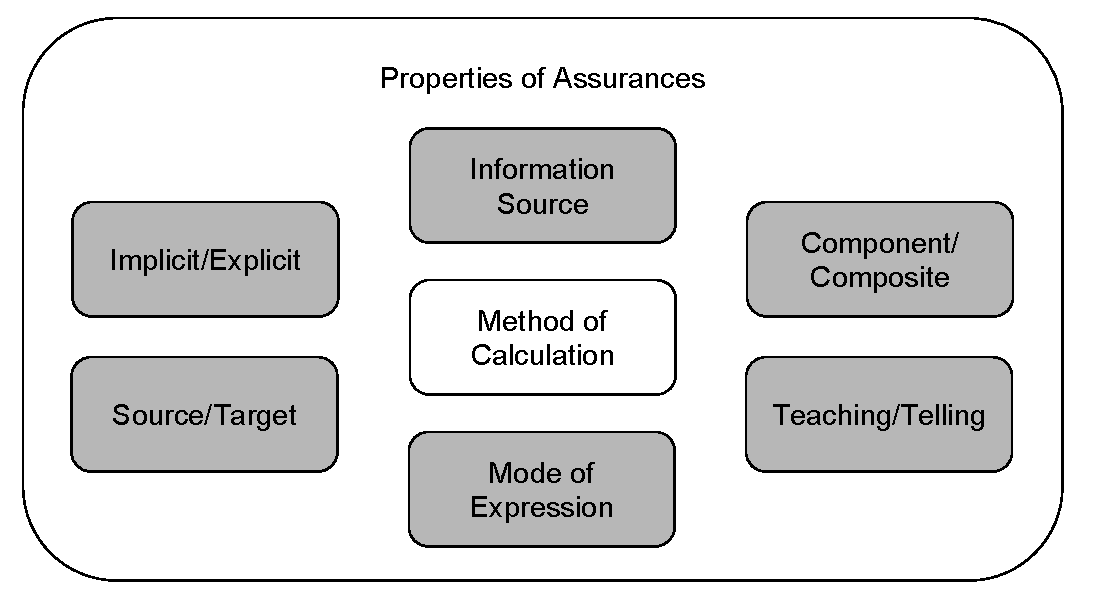
\includegraphics[width=0.6\linewidth]{Figures/Assurance_properties.pdf}
        \caption{All assurances possess at least these properties (others likely exist as well).}
        \label{fig:assurance_classification}
    \end{figure}

    \brettcomm{Discuss the main taxonomy of the survey. Mention that other taxonomies are possible and are mentioned in the future work section\ldots Make clear that our survey is going pursue the taxonomy of algorithms that have been used to calculate assurances}

    Researchers in the fields of AI, ML, data science, and robotics will recognize terms like \emph{interpretable}, \emph{comprehensible}, \emph{transparent}, \emph{verified and validated} (V\&V), \emph{certified}, and \emph{explainable AI}, with respect to the models or performance of a designed AIA. A key claim of this paper is that, \textbf{from a high level, all of these approaches have the same underlying aim: for a user to be able to trust an AIA to operate in a certain way, and (based on that trust) behave appropriately towards the AIA}. These fields have thus each developed mechanisms to assure or calculate assurances that are similar on a fundamental level. 
